\documentclass[]{article}

\usepackage{graphicx}
\usepackage{pdfpages}
\usepackage{amssymb}
\usepackage{caption}
\usepackage{subcaption}
\usepackage{hyperref}
\usepackage{geometry}

%opening
\title{\vspace{-3.0cm}Insertion Sort}
\author{Yori Verbist}

\begin{document}

\maketitle

\section{Theoretisch vs. experiment}
Zoals je in de onderstaande grafieken kan zien bevistigt het experiment de theorie. Rechts is het algorithme te zien op een kleine array en links op een grote. Het kleine verschil bij de kleine rijen heeft te maken met de lagere orde termen (deze termen worden ook weggelaten bij de ~-notatie). Wanneer het aantal te sorteren elementen klein is zal dit dus een groter impact hebben. \newline
Het is ook makkelijk in te zien dat het experiment altijd de theorie gaat bevestigen omdat je er zeker van bent dat er altijd evenveel bewerkingen gaan worden uitgevoerd. Analoog weet je ook dat het niet uitmaakt of de te sorteren elementen verschillend zijn van elkaar of allemaal hetzelfde. Omdat je elke lus alle overige elementen gaat vergelijken met het eerste element van die lus.

\begin{figure}[h!]
	\centering
	\begin{subfigure}[b]{.44\textwidth}
		\centering
		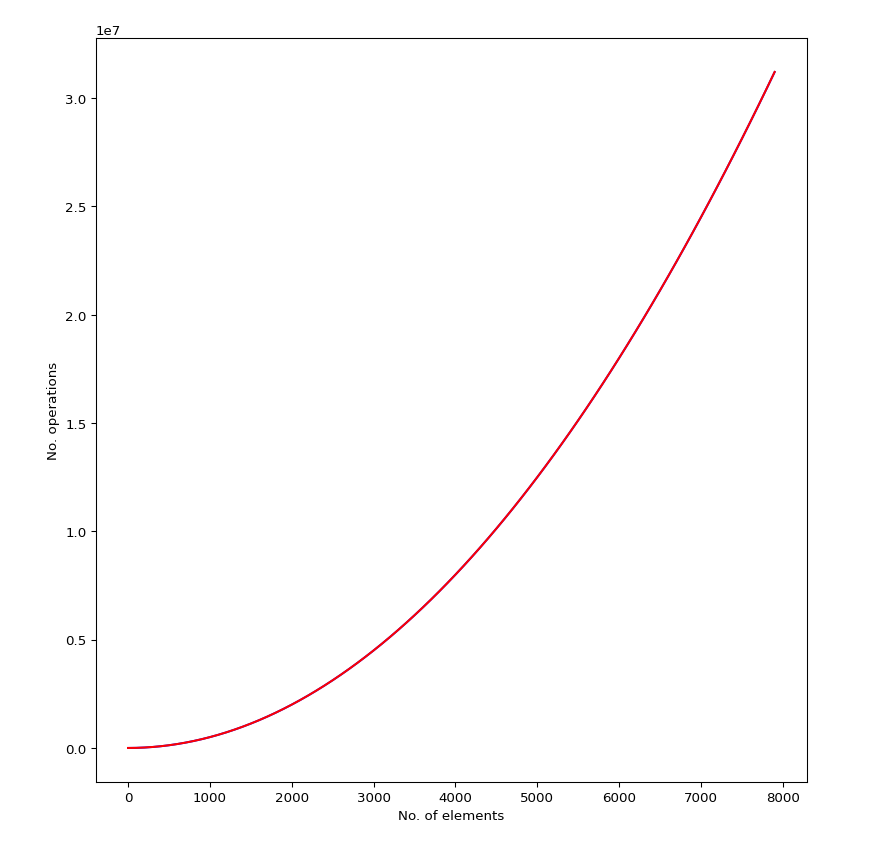
\includegraphics[width=\textwidth]{big}
		\caption{Lijst met 8000 elementen}
	\end{subfigure}
	\hfill
	\begin{subfigure}[b]{.45\textwidth}
		\centering
		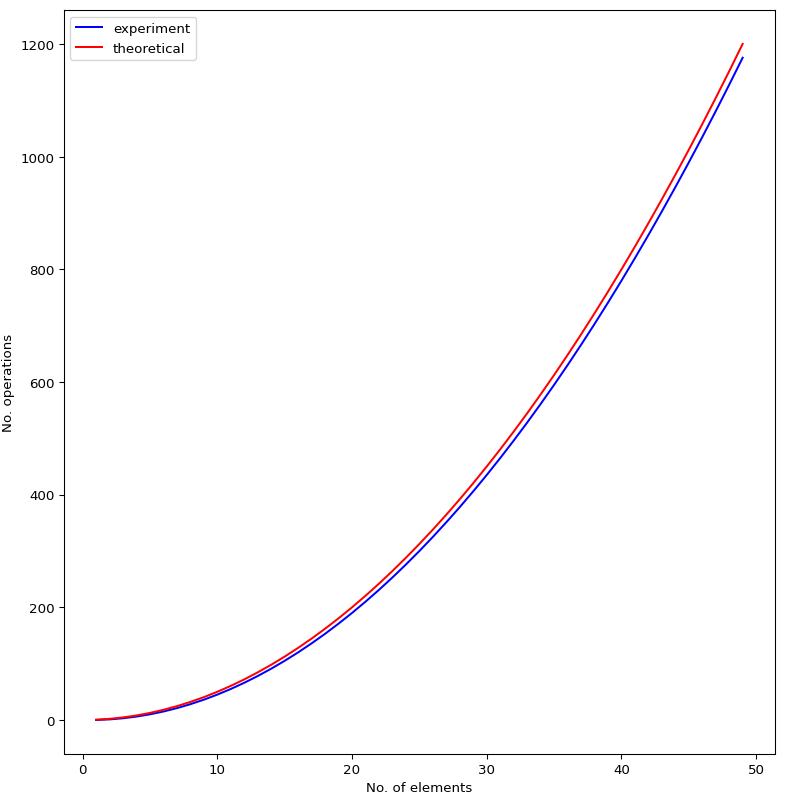
\includegraphics[width=\textwidth]{small}
		\caption{Lijst met 50 elementen}
	\end{subfigure}
\end{figure}


\end{document}
